\documentclass{homework}

\title{Homework 7}
\author{Kevin Evans}
\studentid{11571810}
\date{March 8, 2021}
\setclass{Physics}{461}
\usepackage{amssymb}
%\usepackage{mathtools}
 \usepackage{graphicx}
\usepackage{amsthm}
\usepackage{amsmath}
\usepackage{slashed}
\usepackage{boldline}
\usepackage{physics}
\usepackage[inter-unit-product =\cdot]{siunitx}

\usepackage[makeroom]{cancel}
\usepackage{booktabs}

\usepackage{times}
\usepackage{mhchem}

%\usepackage{calligra}
%\DeclareMathAlphabet{\mathcalligra}{T1}{calligra}{m}{n}
%\DeclareFontShape{T1}{calligra}{m}{n}{<->s*[2.2]callig15}{}
%\newcommand{\scriptr}{\mathcalligra{r}\,}
%\newcommand{\boldscriptr}{\pmb{\mathcalligra{r}}\,}
%\newcommand{\emf}{\mathcal{E}}

\begin{document}
	\maketitle
	\begin{enumerate}
		\item \begin{enumerate}
			\item Presumably because of electron screening. The $p$ and $d$ levels are further than the $s$, and the electrons in $s$ can screen the electric field from the nucleus. As $z$ increases, the nucleus becomes more positively charged and it reduces the effect of the screening, leading to a plateau.
			
			\item Maybe something like this:
		
			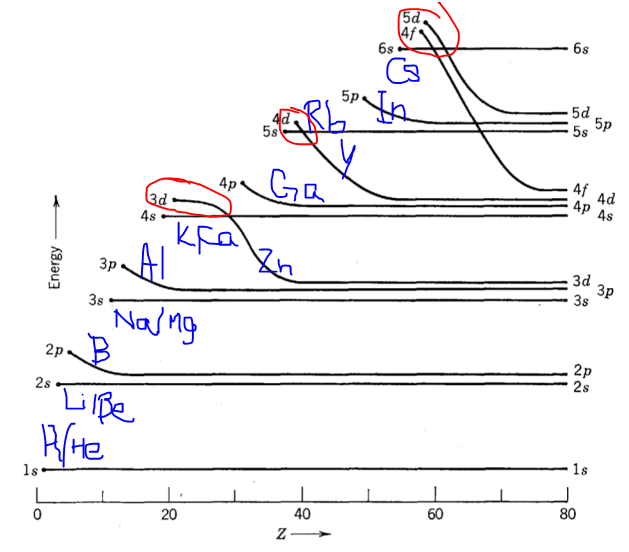
\includegraphics[width=0.7\linewidth]{hw7_1}
			
		\end{enumerate}
		
		\item \begin{enumerate}
			\item Because in the experiment, the X-ray emission is coming from the $K$ series lines, which are the same transitions seen by the sodium atom during absorption spectroscopy.
			\item Presumably because tungsten is a high $Z$ atom, leading to a larger magnetic moment and a larger energy splitting.
			
			\item Because the energy is proportional to $Z^2$ in hydrogen-like states.
			
			\item The $K$ series lines are the lowest ones ($\to 1s$). The $L$ series are the next lowest, $\to 2s/2p$.
			
			\item No? The upper plot has a higher energy value.
		\end{enumerate}
	
		\item \begin{enumerate}
			\item There are four states in the Slater basis, \begin{align*}
				\ket{\alpha \beta}_1 & = \mathcal{A} \ket{\alpha \beta}_a = \ket{\alpha \beta}_a - \ket{\alpha \beta}_{a'}\\
				\ket{\alpha \beta}_2 & = \mathcal{A} \ket{\alpha \beta}_b = \ket{\alpha \beta}_b - \ket{\alpha \beta}_{b'}\\
				\ket{\alpha \beta}_3 & = \mathcal{A} \ket{\alpha \beta}_c = \ket{\alpha \beta}_c - \ket{\alpha \beta}_{c'}\\
				\ket{\alpha \beta}_4 & = \mathcal{A} \ket{\alpha \beta}_d 
				= \ket{\alpha \beta}_d - \ket{\alpha \beta}_{d'}
			\end{align*}
			
			\item The singlet state has an antisymmetric spin function, so the total wavefunction will be \begin{align*}
				\left(\ket{\alpha \beta} + \ket{\beta \alpha}\right) \left(\ket{\uparrow \downarrow} - \ket{\downarrow \uparrow}\right) & = \ket{\alpha \uparrow} \ket{\beta \downarrow} - \ket{\alpha \downarrow} \ket{\beta \uparrow} + \ket{\beta \uparrow} \ket{\alpha \downarrow} - \ket{\beta \downarrow}\ket{\alpha \uparrow} \\ 
					& = \ket{\alpha \beta}_b - \ket{\alpha \beta}_c + \ket{\alpha \beta}_{c'} - \ket{\alpha \beta}_{b'} \\
					& = \ket{\alpha \beta}_2 - \ket{\alpha \beta}_3
			\end{align*}
			For the triplet state, the spinfunction is symmetric, so \begin{align*}
				\left(\ket{\alpha \beta} - \ket{\beta \alpha}\right) \left(\ket{\uparrow \uparrow}\right) & = \ket{\alpha \uparrow} \ket{\beta \uparrow} - \ket{\beta \uparrow}\ket{\alpha \uparrow} \\
					& = \ket{\alpha\beta}_1
				\intertext{I'm guessing the other ones will be $\ket{\alpha\beta}_4$. The last one will be}
				\left(\ket{\alpha \beta} - \ket{\beta \alpha}\right) \left(\ket{\uparrow \downarrow} + \ket{\downarrow \uparrow}\right) & = \ket{\alpha \uparrow}\ket{\beta \downarrow} - \ket{\beta \uparrow} \ket{\alpha \downarrow} + \ket{\alpha \downarrow}\ket{\beta \uparrow} - \ket{\beta \downarrow} \ket{\alpha \uparrow} \\
				& = \ket{\alpha \beta}_2 + \ket{\alpha \beta}_3
			\end{align*}
		
			\item 4 states, but I don't understand Slater stuff well enough to understand what this question is asking me.
			
			\item We need Russell-Saunders coupling because we're dealing with the electron-electron interaction. 
			
			Treating them separately results in $l=l_1 + l_2 = 2$, $s=s_1 + s_2 = 1$. 
			
			\ce{^3 D}, \ce{^1 D}, \ce{^3 P}, \ce{^1 P}, \ce{^3 S}, \ce{^1 S}
			
			For \ce{^3D}, $l=2$ and $s=1$, $m_l = 2, 1, 0, -1, -2$, $m_s = 1, 0, -1$, giving $15$ unique combinations. For $\ce{^1 D}$, $m_s = 0$, giving $5$ combinations.
			
			For the P states, $9$ and $3$. For the S states, $3$ and $1$ combinations.
			
			The sum of all this is $36$ states.
			
			\item This is jj-coupling, right? So this would be needed when there's electron-electron interaction, but for larger atoms with high $Z$.
			
			Each $j_i = \frac{3}{2}, \frac{1}{2}$. This results in a total $j=3,2,1,0$. For $j=3$, $m_j = 0, \pm 1, \pm 2, \pm 3$ with 7 states. For $j=2$, it's 5 states. For $j=1$, it's 3 states. For $j=0$, there's a single state. 

			This is a total of $16$ states.
		\end{enumerate}
	
		\item Omitting the $\hbar$, then we can factor $j_c$ as \begin{align*}
			J_C & = j_c \sqrt{1 + \frac{1}{j_c}}
		\end{align*}
		...not actually sure what to do here. Should I be substituting in $j_a + j_b$ for $j_c$? Or should I just check the inequality with $j_a(j_a + 1)$ and $j_b(j_b + 1)$?
		
		\item \begin{enumerate}
			\item For the $p$ subshell, $\ell = 1$ and the spherical harmonics squared are \begin{align*}
				{Y_{10}}^2 & = \frac{3}{4 \pi} \cos[2](\theta) \\
				{Y_{11}}^2 & = \frac{3}{8 \pi}  \sin[2](\theta)  \\
				{Y_{1(-1)}}^2 & = \frac{3}{8 \pi} \sin[2](\theta)
				\intertext{Summing these,}
				\sum_k {Y_{1k}}^2 & = \frac{3}{4 \pi} \cos[2](\theta) +  2\left(\frac{3}{8 \pi}\right) \sin[2](\theta) \\
					& = \frac{3}{8 \pi}
			\end{align*}
		
			\item For the $d$ shell, \begin{align*}
				{Y_{20}}^2 & = \frac{5}{16 \pi} \left(3 \cos[2](\theta) - 1\right)^2 \\
				{Y_{2 \pm 1}} & = \frac{15}{8 \pi} \left(\cos \theta \sin \theta\right)^2 \\
				{Y_{2 \pm 2}} & = \frac{15}{32 \pi} \sin[4](\theta)
				\intertext{Summing these in WolframAlpha results in}
				\sum_k {Y_{2k}}^2 & = \frac{5}{4 \pi}
			\end{align*}
		\end{enumerate}
		
		\item \begin{enumerate}
			\item $^2 S_{3/2}$: $s=1/2$, $l=0$, $j=3/2$
			
				$^3 D_2$: $s=1$, $l=2$, $j=2$
				
				$^5 P_3$: $s=2$, $l=1$, $j=3$
			
			\item $^2 S_{3/2}$ is impossible, since the total $j$ exceeds $l+s$.
			
		\end{enumerate}
		
		\item Gonna omit the $j$ value to save space on the spectroscopy notation bit,
		
		 \begin{tabular}{ccll}
			\toprule
			$L$ & $S$ & $J$ & Spect. \\
			\midrule
			$5$ & $0$ & $5$ & \ce{^1 H} \\
			$5$ & $1$ & $6$, $5$, $4$ & \ce{^3 H}  \\
			$4$ & $0$ & $4$ &  \ce{^1 G}\\
			$4$ & $1$ & $5, 4, 3$ &  \ce{^3 G} \\
			$3$ & $0$ & $3$ &  \ce{^1 F} \\
			$3$ & $1$ & $4, 3, 2$ &  \ce{^3 F}\\			
			$2$ & $0$ & $2$ &  \ce{^1 D}\\
			$2$ & $1$ & $3, 2, 1$ &  \ce{^3 D}\\
			$1$ & $0$ & $1$ &  \ce{^1 P}\\
			$1$ & $1$ & $2, 1, 0$ &  \ce{^3 P}\\
			\bottomrule
		\end{tabular}
		
		\item \begin{enumerate}
			\item Since the three negative terms ($\epsilon_{321} = \epsilon_{132} = \epsilon_{213}$) squared are just $1$. The other terms squared are $1$, so summing this results in \begin{align*}
				{\epsilon_{ijk}}{\epsilon_{ijk}} & = 6
			\end{align*}
		
			\item There are only two non-zero components when $k=l$, resulting in $2\delta_{kl}$.
		\end{enumerate}
	
		\item Using the determinate form with the Kronecker deltas, 	\begin{align*}
			\varepsilon_{ijk}\varepsilon_{lmn} &= \begin{vmatrix}
				\delta_{il} & \delta_{im} & \delta_{in} \\
				\delta_{jl} & \delta_{jm} & \delta_{jn} \\
				\delta_{kl} & \delta_{km} & \delta_{kn} \\
			\end{vmatrix}
		\intertext{As $i = l$, then the only non-zero term is}
		\varepsilon_{ijk} \varepsilon_{imn} & = \delta_{jm}\delta_{kn} - \delta_{jn} \delta_{km}
		\end{align*}
	
		\item Given the rule provided, \begin{align*}
			\left[\bvec{A} \cross \left(\bvec{B} \cross \bvec{C}\right)\right]_i & = \epsilon_{ijk} A_j \left( \bvec{B} \cross \bvec{C} \right)_k \\
				& = \epsilon_{ijk} A_j \epsilon_{klm} B_l C_m = \epsilon_{kij}  \epsilon_{klm}  A_j B_l C_m \\
				& = \left(\delta_{il} \delta_{jm} - \delta_{im} \delta_{jl} \right)A_j B_l C_m  \\
				& = B_i A_m B_m - C_i A_l B_l \qed
		\end{align*}
	\end{enumerate}
\end{document}